\documentclass[nobib]{tufte-handout}

\usepackage{amssymb}
\usepackage{hyperref}
\usepackage{pgfplots}
\usepackage[activate={true,nocompatibility},final,tracking=true,kerning=true,spacing=true,factor=1100,stretch=10,shrink=10]{microtype}
\usepackage{color}
\usepackage{steinmetz}
\usepackage{placeins}
\usepackage{marginfix}
\usepackage{array}
\usepackage{tikz}
\usepackage{amsmath,amsthm}
\usetikzlibrary{shapes, arrows, positioning, calc}
\usepackage{listings}
\usepackage{forest}
\usepackage{caption}
\usepackage{graphicx}
\usepackage{booktabs}
\usepackage{units}
\usepackage{fancyvrb}
\usepackage{multicol}

\title{ECE 30200 - Probabilistic Methods in Electrical and Computer Engineering}
\author{Zeke Ulrich}

\begin{document}

\maketitle

\tableofcontents

\pagebreak

\section{Background}

The following formulas will be instrumental and may be familar.

\subsection{Series}
\begin{equation}
    \sum_{k=0}^{n} r^k = \frac{1 - r^{n + 1}}{1 - r}
\end{equation}
\begin{equation}
    \sum_{n=1}^{\infty} \frac{1}{n^2} = \frac{\pi^2}{6}
\end{equation}
\begin{equation}
    \sum_{k=1}^{\infty}kr^{k - 1} = \frac{1}{(1 - r)^2}
\end{equation}

\subsection{Combinatorics}
\begin{equation}
    {n\choose k} = \frac{n!}{k!(n - k)!}
\end{equation}
\begin{equation}
    (a + b)^n = \sum_{k=0}^{n} {n\choose k} a^{n - k}b^k
\end{equation}
\begin{equation}
    {n\choose k} + {n\choose k-1} = {n + 1\choose k}
\end{equation}
\begin{equation}
    P(n, k) = \frac{n!}{(n-k)!}
\end{equation}
where $P(n, k)$ is the number of ways to arrange $k$ objects out of $n$ (permutations).
\begin{equation}
    C(n, k) = {n\choose k} = \frac{n!}{k!(n-k)!}
\end{equation}
where $C(n, k)$ is the number of ways to choose $k$ objects out of $n$ (combinations).

\subsection{Approximations}
\begin{align}
    f(x) & = f(a) + f'(a)(x - a) + \frac{f''(a)}{2!}(x - a)^2 + \dots \\
         & = \sum_{n=0}^{\infty} \frac{f^{(n)}(a)}{n!}(x - a)^n
\end{align}
\begin{align}
    1 + x + \frac{x^2}{2!} + \frac{x^3}{3!} + \dots & = \sum_{k=0}^{\infty} \frac{x^k}{k!} \\
                                                    & = e^x
\end{align}
\begin{align}
    \sin(x) & = x - \frac{x^3}{3!} + \frac{x^5}{5!} - \frac{x^7}{7!} + \dots \\
            & = \sum_{n=0}^{\infty} (-1)^n \frac{x^{2n+1}}{(2n+1)!}
\end{align}
\begin{align}
    \cos(x) & = 1 - \frac{x^2}{2!} + \frac{x^4}{4!} - \frac{x^6}{6!} + \dots \\
            & = \sum_{n=0}^{\infty} (-1)^n \frac{x^{2n}}{(2n)!}
\end{align}
\begin{align}
    \ln(1 + x) & = x - \frac{x^2}{2} + \frac{x^3}{3} - \frac{x^4}{4} + \dots \\
               & = \sum_{n=1}^{\infty} (-1)^{n+1} \frac{x^n}{n}
\end{align}

\subsection{Calculus}
\begin{equation}
    \frac{d}{dx} \int_{a}^{x} f(t)\,dt = f(x)
\end{equation}
\begin{equation}
    \int_{a}^{b} f'(x)\,dx = f(b) - f(a)
\end{equation}
\begin{equation}
    \int f(g(x))g'(x)\,dx = \int f(u)\,du
\end{equation}
\begin{equation}
    \int u\,dv = uv - \int v\,du
\end{equation}
\begin{equation}
    \int \frac{1}{(x-a)(x-b)}\,dx = \frac{1}{b-a} \ln\left|\frac{x-a}{x-b}\right| + C
\end{equation}

\subsection{Linear Algebra}
\begin{equation}
    \vec{y} = \beta_1 \vec{x_1} + \beta_2 \vec{x_2} + \cdots + \beta_N \vec{x_N}
\end{equation}
\begin{align}
    \langle \vec{a}, \vec{b} \rangle & = \vec{a}\vec{b}^{T}     \\
                                     & = \sum_{i=1}^{n} a_i b_i
\end{align}
where $\langle \vec{a}, \vec{b} \rangle$ denotes the inner product of vectors $\vec{a}$ and $\vec{b}$.
\begin{equation}
    \|\vec{x}\|_p = \left( \sum_{i=1}^{n} |x_i|^p \right)^{1/p}
\end{equation}
where $\|\vec{x}\|_p$ is the $p$-norm (or $\ell_p$-norm) of vector $\vec{x}$.
\begin{equation}
    \cos(\theta) = \frac{\langle \vec{a}, \vec{b} \rangle}{\|\vec{a}\|_2 \|\vec{b}\|_2}
\end{equation}
where $\theta$ is the angle between vectors $\vec{a}$ and $\vec{b}$.
\begin{equation}
    \hat{\beta} = (\mathbf{X}^T \mathbf{X})^{-1} \mathbf{X}^T \vec{y}
\end{equation}
where $\hat{\beta}$ is the vector of least squares coefficients, $\mathbf{X}$ is the data matrix, and $\vec{y}$ is the target vector.

\section{Formal Definitions}

\subsection{Outcomes}
An \emph{outcome} is the result of some \emph{experiment}.
If that experiment is flipping a coin, the outcome is either
heads or tails. We could express the outcome of heads as $H$,
and the outcome of tails as $T$. The set of all possible
outcomes for an experiment is known as a sample space and is
denoted by $\Omega$. In this case $\Omega = \{H, T\}$.

\subsection{Events}
An \emph{event} $F$ is a subset of the probability space $\Omega$.
The formal definitions of probability are expressed with set
notation. So the event where we have neither heads nor tails is
written as $\{\}$. The event of heads could be expressed as
$\{H\}$, and the event of tails could be expressed as $\{T\}$.
The event of either heads or tails is $\{\Omega\}$.

\subsection{Probability Laws}
A \emph{probability law} is a function $P$ that maps an event $A$
to a real number in $[0, 1]$. For the coin example, the probability
law might be $P(\{\}) = 0$, $P(\{H\}) = 0.5$, $P(\{T\}) = 0.5$, and
$P(\{\Omega\}) = 1$. A probability law must satisfy three axioms:
\begin{enumerate}
    \item Non-negativity: $P(A) \geq 0 \forall A \in F$
    \item Normalization: $P(\Omega) = 1$
    \item Additivity: For any disjoint subsets $\{A_1, A_2, \dots\}$,
          it holds that
          \[P\left[\bigcup_{n=1}^{\infty}A_n\right] = \sum_{n=1}^{\infty}P\left[A_n\right]\]
\end{enumerate}

\subsection{Probability Space}
A probability space is a triplet $\Omega, F, P$.

\subsection{Probability Properties}
\begin{equation}
    P\left[A \cup B\right] = P\left[A\right] + P\left[B\right] - P\left[A \cap B\right]
\end{equation}
\begin{equation}
    P\left[A \cup B\right] \leq P\left[A\right] + P\left[B\right]
\end{equation}
\begin{equation}
    A \subseteq B \implies P\left[A\right] \leq P\left[B\right]
\end{equation}
\begin{equation}
    P\left[A | B\right] = \frac{P[A \cap B]}{P[B]}
\end{equation}

\subsection{Probability Properties}
\begin{equation}
    P\left[A \cup B\right] = P\left[A\right] + P\left[B\right] - P\left[A \cap B\right]
\end{equation}
\begin{equation}
    P\left[A \cup B\right] \leq P\left[A\right] + P\left[B\right]
\end{equation}
\begin{equation}
    A \subseteq B \implies P\left[A\right] \leq P\left[B\right]
\end{equation}
\begin{equation}
    P\left[A | B\right] = \frac{P[A \cap B]}{P[B]}
\end{equation}

Outcomes are statistically \emph{independent} if
$P(A|B) = P(A)$ (assuming P(B) > 0), or
equivalently $P(A \cap B) = P(A)P(B)$.
\include{chapters/discreterandomvariables}
\section{Continuous Random Variables}

A \emph{continuous random variable} is
analogous to the discrete case. Recall that
a probability is just a size of a set.
It's easy to find the size of a discrete set
because you can just count elements, but for
an uncountable set new methods are needed. Luckily
the intution for continuous random variables is
intuitive, it's still just the size of a set $A$
relative to $\Omega$.
\begin{figure}[h]
    \centering
    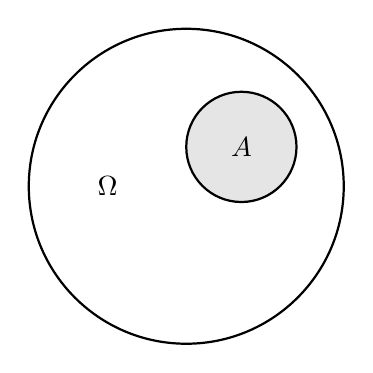
\begin{tikzpicture}[scale=1]
        \draw[thick] (0,0) circle (2cm);
        \node at (-1,0) {$\Omega$};
        \draw[thick, fill=gray!20] (0.7,0.5) circle (0.7cm);
        \node at (0.7,0.5) {$A$};
    \end{tikzpicture}
    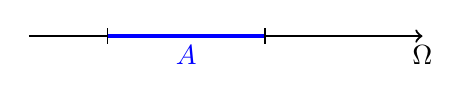
\begin{tikzpicture}[scale=1]
        \draw[thick,->] (0,0) -- (5,0);
        \node[below] at (5,0) {$\Omega$};
        \draw[very thick,blue] (1,0) -- (3,0);
        \node[below,blue] at (2,0) {$A$};
        \draw (1,0.1) -- (1,-0.1);
        \draw (3,0.1) -- (3,-0.1);
    \end{tikzpicture}
    \caption{Continuous random variables}
\end{figure}
Formally, if each event in A is equally likely, then
\begin{equation}
    P[\{x \in A\}] = \frac{\int_{A}dx}{|\Omega|}
\end{equation}
If we relax the assumption of equiprobability, then
more generally
\begin{equation}
    P[\{x\in A\}] = \int_{A} f_X(x) dx
\end{equation}
$f_X(x)$ is called the \emph{probability density function} (PDF).
It is analogous to the probability mass function.

Formally, a probability density function
is a mapping $f_X: \Omega \implies \Re$,
with the following properties:
\begin{itemize}
    \item Non-negativity: $f_X(x) \geq 0 \forall x \in \Omega$
    \item Unity: $\int_{\Omega} f_X(x)dx = 1$
    \item Measure of a set: $P[\{x \in A\}] = \int_{A}f_X(x) dx$
\end{itemize}

We can express a PDF in terms of a PMF
with a train of delta functions like so:
\begin{equation}
    f_X(x) = \sum_{x_k \in \Omega} p_X(x_k) \delta(x - x_k)
\end{equation}

We can also define the probability density
function as the derivative of the CDF, like so:
\begin{equation}
    f_X(x) = \frac{d}{dx}p(X \leq x)
\end{equation}

The expectation of a continuous random variable is
\begin{equation}
    E[X] = \int_{\Omega} xf_X(x)dx
\end{equation}

Properties of the expectation for continuous
random variables:
\begin{itemize}
    \item $E[aX] = aE[X]$
    \item $E[X+a] = E[X] + a$
    \item $E[aX+b] = aE[X] + b$
\end{itemize}

A random variable $X$ has an expectation
if it is absolutely integrable,
\begin{equation}
    E[|X|] = \int_{\Omega} |x|f_X(x)dx < \infty
\end{equation}

The variance of a continuous random variable
$X$ is
\begin{align}
    Var[X] & = E[(X-\mu)^2]                    \\
           & = \int_{\Omega} (x-\mu)^2f_X(x)dx \\
           & = E[X^2] - \mu^2
\end{align}

A continuous \emph{uniform random variable}
has a PDF of
\begin{equation}
    f_X(x) = \begin{cases}
        \frac{1}{b-a} & a \leq x \leq b \\
        0             & \text{else}
    \end{cases}
\end{equation}
We write
\begin{equation}
    X \sim Uniform(a,b)
\end{equation}
to mean that $X$ is drawn from a uniform
distribution on an interval $[a, b]$.
It has a CDF given by
\begin{equation}
    F_X(x) = \begin{cases}
        0               & a < a           \\
        \frac{x-a}{b-a} & a \leq x \leq b \\
        1               & x > b
    \end{cases}
\end{equation}
If $X \sim Uniform(a,b)$ then
\begin{align}
    E[X]   & = \frac{a + b}{2}      \\
    Var[X] & = \frac{(b - a)^2}{12}
\end{align}

A continuous \emph{exponential random variable}
has a PDF of
\begin{equation}
    f_X(x) = \begin{cases}
        \lambda e^{-\lambda x} & x \geq 0    \\
        0                      & \text{else}
    \end{cases}
\end{equation}
\marginnote{An exponential random variable
    is the interarrival time between two consecutive
    Poisson events}
We write
\begin{equation}
    X \sim Exponential(\lambda)
\end{equation}
to mean that $X$ is drawn from an
exponential distribution of parameter
$\lambda$. It has a CDF given by
\begin{equation}
    F_X(x) = 1 - e^{-\lambda x}
\end{equation}
If $X \sim Exponential(\lambda)$, then
\begin{align}
    E[X]   & = \frac{1}{\lambda}   \\
    Var[X] & = \frac{1}{\lambda^2}
\end{align}

A \emph{Gaussian random variable} is a
random variable $X$ such that its PDF
is
\begin{equation}
    f_X(x) = \frac{1}{\sqrt{2\pi \sigma^2}}\exp\left(-\frac{(x-\mu)^2}{2\sigma^2}\right)
\end{equation}
We write
\begin{equation}
    X \sim Gaussian(\mu, \sigma^2)
\end{equation}
or
\begin{equation}
    X \sim \mathcal{N}\left(\mu, \sigma^2\right)
\end{equation}
to mean that $X$ is drawn from a Gaussian
of parameter $(\mu, \sigma^2)$.
If $X \sim \mathcal{N}(\mu, \sigma^2)$, then
\begin{align}
    E[X]   & = \mu      \\
    Var[X] & = \sigma^2
\end{align}

The \emph{standard Gaussian} random variable has a
PDF given by
\begin{equation}
    f_X(x) = \frac{1}{\sqrt{2\pi}} e^{-\frac{x^2}{2}}
\end{equation}
The CDF of the standard Gaussian is defined
as the $\Phi$ function.
\begin{equation}
    \Phi(x) = \frac{1}{\sqrt{2\pi}}\int_{-\infty}^{\infty} e^{-\frac{t^2}{2}}dt
\end{equation}
The CDF of the standard Gaussian is related to the
\emph{error function}, which is defined as
\begin{equation}
    \text{erf}(x) = \frac{2}{\sqrt{\pi}} \int_{0}^{x} e^{-t^2} dt
\end{equation}
by the relation
\begin{equation}
    \Phi(x) = \frac{1}{2} \left(1 + \text{erf}\left(\frac{x}{\sqrt{2}}\right)\right)
\end{equation}
The CDF of an arbitrary Gaussian is related via
the transformation
\begin{equation}
    F_X(x) = \phi\left(\frac{x - \mu}{\sigma}\right)
\end{equation}

In addition to mean and variance, we introduce
two more useful quantities, \emph{skewness} and
\emph{kurtosis}.
\begin{align}
    E\left[X\right]                                   & = \mu      \\
    E\left[(X - \mu)^2\right]                         & = \sigma^2 \\
    E\left[\left(\frac{X-\mu}{\sigma}\right)^3\right] & = \gamma   \\
    E\left[\left(\frac{X-\mu}{\sigma}\right)^4\right] & = \kappa
\end{align}
\marginnote{\emph{Excess kurtosis} is defined
    as $\kappa - 3$}

Skewness measures the asymmetry of a
distribution. A Gaussian distribution has
skewness 0. Kurtosis measures how heavy-tailed
the distribution is. If the kurtosis is
positive, then the tails decay faster than a
Gaussian. If the kurtosis is negative, then
the distribution has a tail that
decays more slowly than a Gaussian.

The definition of a CDF is
\begin{equation}
    F_X(x) = P[X \leq x]
\end{equation}
\begin{figure}
    \centering
    \includegraphics[scale=0.5]{images/normal_distribution_plot.png}
    \caption{PDF and CDF}
\end{figure}
Let $X$ be a continuous random variable. if the CDF
$F_X$ is continuous at any $a\leq x \leq b$, then
\begin{equation}
    P[a \leq X \leq b] = F_X(b) - F_X(a)
\end{equation}
A function $F_X(x)$ is said to be left
continuous if at $x=b$
\begin{equation}
    F_X(b) - \lim_{h\implies 0} F_X(b-h)
\end{equation}
and right continuous if
\begin{equation}
    F_X(b) - \lim_{h\implies 0} F_X(b+h)
\end{equation}
and continuous if $F_X(x)$ is both left
and right continuous.
All CDFs are right continuous.

For any random variable $X$, discrete or continuous,
\begin{equation}
    P[X=b] = \begin{cases}
        F_X(b) - F_X(b^-) & \text{if $F_X$ is discontinuous at $x=b$} \\
        0                 & \text{else}
    \end{cases}
\end{equation}

The PDf is the derivative of the CDF.
\begin{equation}
    f_X(x) = \frac{d}{dx} \int_{-\infty}^{x} f_X(t)dt
\end{equation}
provided $F_X$ is differentiable at $x$. If not, then
\begin{equation}
    f_X(x) = F_X(x) - \lim_{h\implies 0} F_X(x-h)
\end{equation}

Let $X$ be a continuous random variable with PDF
$f_X$. The median of $X$ is a point $c \in \Re$ such that
\begin{equation}
    \int_{-\infty}^{c} f_X(x) dx = \int_{c}^{\infty}f_X(x) dx
\end{equation}

Let $X$ be a continuous random variable. The mode is
the point $c$ such that $f_X(x)$ attains the maximum.
\begin{equation}
    x = \text{argmax}_{x \in \Omega} f_X(x)
\end{equation}

The mean $E[X]$ can be computed from
$F_X$ as
\begin{equation}
    E[X] = \int_{0}^{\infty} (1-F_X(t))dt
\end{equation}
\section{Functions of Random Variables}

In general, given some random variable
$X$, we may wish to know the properties
of $Y = g(X)$, where $g$ is a function.

To find the PDF of $Y = g(X)$, the first
step is to find the CDF
\begin{equation}
    F_Y(y) = F_X(g^{-1}(y))
\end{equation}
The next step is to find the PDF, given by
\begin{equation}
    f_Y(y) = \left(\frac{d}{dy}g^{-1}(y)\right)f_X(g^{-1}(y))
\end{equation}

Suppose $X$ is an exponential random variable
with parameter $\lambda$, and let $Y  = aX + b$.
Then the CDF and PDF of Y are respectively
\begin{align}
    F_Y(y) & = 1 - e^{-\frac{\lambda}{a}(y - b)}, y \geq b              \\
    f_Y(y) & = \frac{\lambda}{a}e^{-\frac{\lambda}{a}(y - b)}, y \geq b
\end{align}

Suppose $X$ is a uniform random variable in $\left[a, b\right], a > 0$,
and let $Y = X^2$. Then the CDF and PDF of Y are respectively
\begin{align}
    F_Y(y) & = \frac{\sqrt{y} - a}{b - a}, a^2 \leq y \leq b^2 \\
    f_Y(y) & = \frac{1}{\sqrt{y}(b - a)}, a^2 \leq y \leq b^2
\end{align}

To generate random numbers from an arbitrary
distribution $F_X$, first generate a random
number $U \sim Uniform(0,1)$, then let
$Y = F^{-1}_X(U)$. The distribution of $Y$ is
$F_X$.

Given two random variables $X$ and $Y$, the
PDF of $Z = X + Y$ is given by
\begin{align}
    f_Z(z) & = f_X(x) * f_Y(y)                          \\
           & = \int_{-\infty}^{\infty} f_X(z-y)f_Y(y)dy
\end{align}

As more random variablaes are summed, their
distribution (no matter the distribution) of each
individual variable) approaches a Gaussian.

Let $X_1 \sim \text{Gauss}(\mu_1, \sigma_1^2)$ and
$X_2 \sim \text{Gauss}(\mu_2, \sigma_2^2)$, then
\begin{equation}
    X_1 + X_2 \sim \text{Gauss}\left( \mu_1 + \mu_2, \sigma_1^2 + \sigma_2^2 \right)
\end{equation}

\appendix

\section{Reference}
\setcounter{equation}{0}

\subsection{Series}
\begin{equation}
    \sum_{k=0}^{n} r^k = \frac{1 - r^{n + 1}}{1 - r}
\end{equation}
\begin{equation}
    \sum_{n=1}^{\infty} \frac{1}{n^2} = \frac{\pi^2}{6}
\end{equation}
\begin{equation}
    \sum_{k=1}^{\infty}kr^{k - 1} = \frac{1}{(1 - r)^2}
\end{equation}

\subsection{Combinatorics}
\begin{equation}
    {n\choose k} = \frac{n!}{k!(n - k)!}
\end{equation}
\begin{equation}
    (a + b)^n = \sum_{k=0}^{n} {n\choose k} a^{n - k}b^k
\end{equation}
\begin{equation}
    {n\choose k} + {n\choose k-1} = {n + 1\choose k}
\end{equation}
\begin{equation}
    P(n, k) = \frac{n!}{(n-k)!}
\end{equation}
where $P(n, k)$ is the number of ways to arrange $k$ objects out of $n$ (permutations).
\begin{equation}
    C(n, k) = {n\choose k} = \frac{n!}{k!(n-k)!}
\end{equation}
where $C(n, k)$ is the number of ways to choose $k$ objects out of $n$ (combinations).

\subsection{Approximations}
\begin{align}
    f(x) & = f(a) + f'(a)(x - a) + \frac{f''(a)}{2!}(x - a)^2 + \dots \\
         & = \sum_{n=0}^{\infty} \frac{f^{(n)}(a)}{n!}(x - a)^n
\end{align}
\begin{align}
    1 + x + \frac{x^2}{2!} + \frac{x^3}{3!} + \dots & = \sum_{k=0}^{\infty} \frac{x^k}{k!} \\
                                                    & = e^x
\end{align}
\begin{align}
    \sin(x) & = x - \frac{x^3}{3!} + \frac{x^5}{5!} - \frac{x^7}{7!} + \dots \\
            & = \sum_{n=0}^{\infty} (-1)^n \frac{x^{2n+1}}{(2n+1)!}
\end{align}
\begin{align}
    \cos(x) & = 1 - \frac{x^2}{2!} + \frac{x^4}{4!} - \frac{x^6}{6!} + \dots \\
            & = \sum_{n=0}^{\infty} (-1)^n \frac{x^{2n}}{(2n)!}
\end{align}
\begin{align}
    \ln(1 + x) & = x - \frac{x^2}{2} + \frac{x^3}{3} - \frac{x^4}{4} + \dots \\
               & = \sum_{n=1}^{\infty} (-1)^{n+1} \frac{x^n}{n}
\end{align}

\subsection{Calculus}
\begin{equation}
    \frac{d}{dx} \int_{a}^{x} f(t)\,dt = f(x)
\end{equation}
\begin{equation}
    \int_{a}^{b} f'(x)\,dx = f(b) - f(a)
\end{equation}
\begin{equation}
    \int f(g(x))g'(x)\,dx = \int f(u)\,du
\end{equation}
\begin{equation}
    \int u\,dv = uv - \int v\,du
\end{equation}
\begin{equation}
    \int \frac{1}{(x-a)(x-b)}\,dx = \frac{1}{b-a} \ln\left|\frac{x-a}{x-b}\right| + C
\end{equation}

\subsection{Linear Algebra}
\begin{equation}
    \vec{y} = \beta_1 \vec{x_1} + \beta_2 \vec{x_2} + \cdots + \beta_N \vec{x_N}
\end{equation}
\begin{align}
    \langle \vec{a}, \vec{b} \rangle & = \vec{a}\vec{b}^{T}     \\
                                     & = \sum_{i=1}^{n} a_i b_i
\end{align}
where $\langle \vec{a}, \vec{b} \rangle$ denotes the inner product of vectors $\vec{a}$ and $\vec{b}$.
\begin{equation}
    \|\vec{x}\|_p = \left( \sum_{i=1}^{n} |x_i|^p \right)^{1/p}
\end{equation}
where $\|\vec{x}\|_p$ is the $p$-norm (or $\ell_p$-norm) of vector $\vec{x}$.
\begin{equation}
    \cos(\theta) = \frac{\langle \vec{a}, \vec{b} \rangle}{\|\vec{a}\|_2 \|\vec{b}\|_2}
\end{equation}
where $\theta$ is the angle between vectors $\vec{a}$ and $\vec{b}$.
\begin{equation}
    \hat{\beta} = (\mathbf{X}^T \mathbf{X})^{-1} \mathbf{X}^T \vec{y}
\end{equation}
where $\hat{\beta}$ is the vector of least squares coefficients, $\mathbf{X}$ is the data matrix, and $\vec{y}$ is the target vector

\subsection{Set Theory}
\begin{equation}
    A \setminus B = \{ x \mid x \in A \text{ and } x \notin B \}
\end{equation}
\begin{itemize}
    \item \textbf{Commutativity:}
          \begin{align}
              A \cup B & = B \cup A \\
              A \cap B & = B \cap A
          \end{align}
    \item \textbf{Associativity:}
          \begin{align}
              (A \cup B) \cup C & = A \cup (B \cup C) \\
              (A \cap B) \cap C & = A \cap (B \cap C)
          \end{align}
    \item \textbf{Distributivity:}
          \begin{align}
              A \cup (B \cap C) & = (A \cup B) \cap (A \cup C) \\
              A \cap (B \cup C) & = (A \cap B) \cup (A \cap C)
          \end{align}
    \item \textbf{Identity:}
          \begin{align}
              A \cup \emptyset & = A \\
              A \cap \Omega    & = A
          \end{align}
    \item \textbf{Complement:}
          \begin{align}
              A \cup A^c & = \Omega    \\
              A \cap A^c & = \emptyset
          \end{align}
\end{itemize}

\subsection{Probability Laws}
\begin{enumerate}
    \item Non-negativity: $P(A) \geq 0 \forall A \in F$
    \item Normalization: $P(\Omega) = 1$
    \item Additivity: For any disjoint subsets $\{A_1, A_2, \dots\}$,
          it holds that
          \[P\left[\bigcup_{n=1}^{\infty}A_n\right] = \sum_{n=1}^{\infty}P\left[A_n\right]\]
\end{enumerate}

\subsection{Probability Properties}
\begin{equation}
    P\left[A \cup B\right] = P\left[A\right] + P\left[B\right] - P\left[A \cap B\right]
\end{equation}
\begin{equation}
    P\left[A \cup B\right] \leq P\left[A\right] + P\left[B\right]
\end{equation}
\begin{equation}
    A \subseteq B \implies P\left[A\right] \leq P\left[B\right]
\end{equation}

\subsection{Discrete Random Variables}
\begin{align}
    E[g(X)]        & = \sum_{x} g(x)p_X(x) \\
    E[g(X) + h(X)] & = E[g(X)] + E[h(X)]   \\
    E[cX]          & = cE[X]               \\
    E[X + c]       & = E[X] + c
\end{align}
\begin{align}
    \text{Var}[X] & = E\left[(X-\mu)^2\right] \\
                  & = E[X^2] - (E[X])^2
\end{align}
\begin{equation}
    P[X\in A | Y = y] = \sum_{x\in A} p_{X|Y}(x|y)
\end{equation}
\begin{align}
    P[X \in A] & = \sum_{x \in A} \sum_{y \in \Omega_Y} p_{X|Y}(x|y)p_Y(y) \\
               & = \sum_{y\in \Omega_Y} P[X\in A|Y = y]p_Y(y)
\end{align}
\begin{equation}
    E[X|Y=y] = \sum_{x} xp_{X|Y}(x|y)
\end{equation}
\begin{equation}
    E[X] = \sum_{y}E[X|Y=y]p_Y(y)
\end{equation}
\begin{equation}
    F_{X,Y}(x,y) = P\left[X \leq x \cap Y \leq y\right]
\end{equation}
\begin{equation}
    F_{X,Y}(x,y) = \sum_{y'\leq y}\sum_{x' \leq x} p_{X,Y}(x',y')
\end{equation}
\begin{equation}
    \text{Cov}(X, Y) = E[XY] - E[X]E[Y]
\end{equation}
\begin{equation}
    \rho = \frac{\text{Cov}(X, Y)}{\sqrt{\text{Var}(X)\text{Var}(Y)}}
\end{equation}

\subsection{Continuous Random Variables}
Conditions of a PDF $f_X$:
\begin{itemize}
    \item Non-negativity: $f_X(x) \geq 0 \forall x \in \Omega$
    \item Unity: $\int_{\Omega} f_X(x)dx = 1$
    \item Measure of a set: $P[\{x \in A\}] = \int_{A}f_X(x) dx$
\end{itemize}
\begin{equation}
    f_X(x) = \frac{d}{dx}p(X \leq x)
\end{equation}
\begin{align}
    E[g(X)]        & = \int_{\Omega} g(x)p_X(x) \\
    E[g(X) + h(X)] & = E[g(X)] + E[h(X)]        \\
    E[cX]          & = cE[X]                    \\
    E[X + c]       & = E[X] + c
\end{align}
\begin{align}
    \text{Var}[X] & = E\left[(X-\mu)^2\right] \\
                  & = E[X^2] - (E[X])^2
\end{align}
\begin{equation}
    \Phi(x) = \frac{1}{\sqrt{2\pi}}\int_{-\infty}^{\infty} e^{-\frac{t^2}{2}}dt
\end{equation}
All CDFs are monotonically increasing, and additionally right continuous. That is,
\begin{equation}
    F_X(b) = \lim_{h\implies 0} F_X(b+h)
\end{equation}
\begin{equation}
    P[X=b] = \begin{cases}
        F_X(b) - F_X(b^-) & \text{if $F_X$ is discontinuous at $x=b$} \\
        0                 & \text{else}
    \end{cases}
\end{equation}
\begin{equation}
    f_X(x) = \frac{d}{dx} \int_{-\infty}^{x} f_X(t)dt
\end{equation}
provided $F_X$ is differentiable at $x$. If not, then
\begin{equation}
    f_X(x) = F_X(x) - \lim_{h\implies 0} F_X(x-h)
\end{equation}
Let $X$ be a continuous random variable with PDF
$f_X$. The median of $X$ is a point $c \in \Re$ such that
\begin{equation}
    \int_{-\infty}^{c} f_X(x) dx = \int_{c}^{\infty}f_X(x) dx
\end{equation}
Let $X$ be a continuous random variable. The mode is
the point $c$ such that $f_X(x)$ attains the maximum.
\begin{equation}
    x = \text{argmax}_{x \in \Omega} f_X(x)
\end{equation}
The mean $E[X]$ can be computed from
$F_X$ as
\begin{equation}
    E[X] = \int_{0}^{\infty} (1-F_X(t))dt
\end{equation}
\begin{equation}
    E[g(X,Y)] = \int_{y\in \Omega_y}\int_{x\in \Omega_x} g(x,y) f_{X,Y}(x,y)dxdy
\end{equation}
\begin{equation}
    \text{Var}[X+Y] = \text{Var}[X] + 2\text{Cov}(X,Y) + \text{Var}[Y]
\end{equation}
\begin{equation}
    f_{X|Y}(x|y) = \frac{f_{X,Y}(x,y)}{f_Y(y)}
\end{equation}
\begin{equation}
    P[X \in A | Y=y] = \int_{A} f_{X|Y}(x|y)dx
\end{equation}
\begin{equation}
    P[X\in A] = \int_{\Omega_Y} P[X\in A|Y = y]f_Y(y)dy
\end{equation}
\begin{equation}
    E[X|Y=y] = \int_{-\infty}^{\infty}xf_{X|Y}(x|y)dx
\end{equation}
\begin{align}
    E[X] & = \int_{-\infty}^{\infty} E[X|Y=y]f_Y(y)dy \\
         & = E_Y[E_{X|Y}[X|Y]]
\end{align}
\begin{equation}
    \text{Cov}(X,Y) = 0 \implies \text{Corr}(X,y) = 0
\end{equation}

\subsection{Functions of Random Variables}
To find the PDF of $Y = g(X)$, the first
step is to find the CDF
\begin{equation}
    F_Y(y) = F_X(g^{-1}(y))
\end{equation}
The next step is to find the PDF, given by
\begin{equation}
    f_Y(y) = \left(\frac{d}{dy}g^{-1}(y)\right)f_X(g^{-1}(y))
\end{equation}
Given two random variables $X$ and $Y$, the
PDF of $Z = XY$ is given by
\begin{equation}
    f_Z(z) = \int_{-\infty}^{\infty} \frac{1}{|y|} f_X(\frac{z}{y}) f_Y(y) dy
\end{equation}
The PDF of $Z = X - Y$ is given by
\begin{equation}
    f_Z(z) = \int_{-\infty}^{\infty} f_X(z + y) f_Y(y) \, dy
\end{equation}
The PDF of $Z = \frac{X}{Y}$ is given by
\begin{equation}
    f_Z(z) = \int_{-\infty}^{\infty} |y| \, f_X(z y) f_Y(y) \, dy
\end{equation}
The PDF of $Z = X + Y$ is given by
\begin{align}
    f_Z(z) & = f_X(x) * f_Y(y)                          \\
           & = \int_{-\infty}^{\infty} f_X(z-y)f_Y(y)dy
\end{align}

\end{document}